\documentclass[10pt, twoside, openany]{book}

\usepackage[a4paper, top=2.5cm, bottom=2.5cm, left=3cm, right=3cm]{geometry}
\usepackage[italian]{babel}
\usepackage{graphicx}
\usepackage{fancyhdr}
\usepackage[Lenny]{fncychap}
\usepackage{frontespizio}

\pagestyle{fancy}
\fancyhead{}
\fancyhead[LE]{\rightmark\hfill\leftmark}
\fancyhead[RO]{\leftmark\hfill\rightmark}

\begin{document}
\begin{frontespizio}
\Universita{Roma Tor Vergata}
\Dipartimento{Ingegneria Civile e Ingegneria dell'Informazione}
\Corso{Ingegneria Informatica}
\Annoaccademico{2023/2024}
\Titolo{Titolo della tesi}
\Candidato[0316179]{Matteo Fanfarillo}
\Relatore{Giuseppe Bianchi}
\Correlatore{Francesco Gringoli}
\Logo{logo.png}
\end{frontespizio}

\begin{flushright}
\null\vspace{\stretch{1}}
\textit{Citazione}
\vspace{\stretch{2}}\null
\end{flushright}

\tableofcontents
\listoffigures
\listoftables

\chapter{Introduzione}
Qui bisogna scrivere l'introduzione.
\begin{figure}
  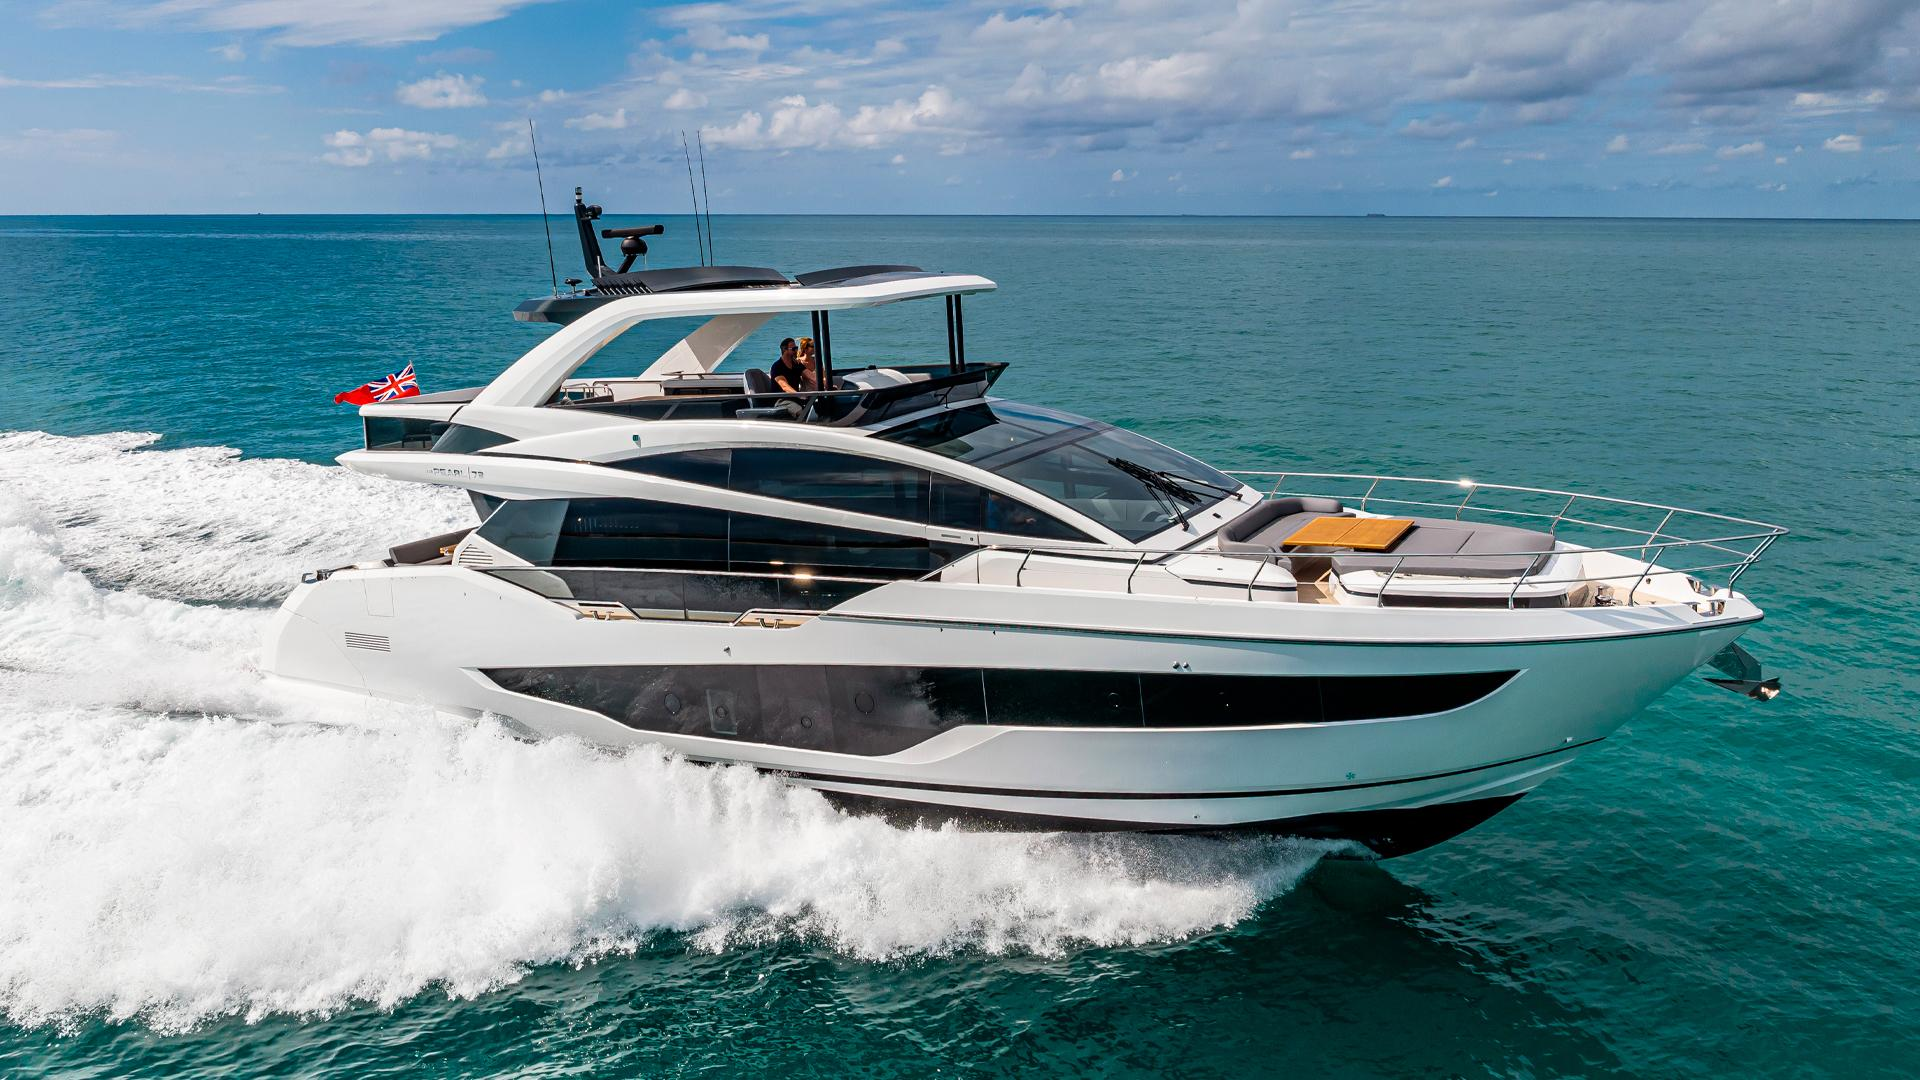
\includegraphics[width=\linewidth]{boat.jpeg}
  \caption{A boat.}
  \label{fig:boat1}
\end{figure}
Figure \ref{fig:boat1} shows a boat.

\chapter{Nuovo capitolo}
\section{Sezione}
This is where you tell people why they should bother reading your article.

\subsection{Sottosezione}
This is the section that is invariably much longer than it should be, and
where everyone tries to impress peers about how easy it is to locate various
references in online databases.

\section{Altra sezione}
Not much of a paper, but it's a start.

\section{Per una nuova pagina}
Riga.\\
Ancora riga.\\
Ancora riga.\\
Ancora riga.\\
Ancora riga.\\
Ancora riga.\\
Ancora riga.\\
Ancora riga.\\
Ancora riga.\\
Ancora riga.\\
Ancora riga.\\
Ancora riga.\\
Ancora riga.\\
Ancora riga.\\
Ancora riga.\\
Ancora riga.\\
Ancora riga.\\
Ancora riga.\\
Ancora riga.\\
Ancora riga.\\
Ancora riga.\\
Ancora riga.\\
Ancora riga.\\
Ancora riga.\\
Ancora riga.\\
Ancora riga.\\
Ancora riga.\\
Ancora riga.\\
Ancora riga.\\
Ancora riga.\\
Ancora riga.

\chapter{Conclusione}
Qui bisogna scrivere la conclusione.\\
\begin{table}[h!]
  \begin{center}
    \caption{Your first table.}
    \label{tab:table1}
    \begin{tabular}{l|c|r} % <-- Alignments: 1st column left, 2nd middle and 3rd right, with vertical lines in between
      \textbf{Value 1} & \textbf{Value 2} & \textbf{Value 3}\\
      $\alpha$ & $\beta$ & $\gamma$ \\
      \hline
      1 & 1110.1 & a\\
      2 & 10.1 & b\\
      3 & 23.113231 & c\\
    \end{tabular}
  \end{center}
\end{table}

\chapter*{Bibliografia}
Qui bisogna scrivere la bibliografia.

\chapter*{Ringraziamenti}
Qui bisogna scrivere i ringraziamenti.

\end{document}